\documentclass[a4paper,12pt]{article}
\usepackage{amsthm}
\usepackage{hyperref}
\usepackage{amsmath}
\usepackage[T1]{fontenc}
\newcommand{\define}[2]{\label{#1}\textbf{\textsc{#1:}}\quad#2\\}
\usepackage{amssymb}
\usepackage{graphicx}
\graphicspath{ {pics/} }
\begin{document}
\title{EE102A Notes}
\author{Michael Uttmark}
\date{\today{}}
\maketitle
\section{Signals and Systems}
\define{Signal}{A function of an independent variable. The dimension of a signal is determined by dimension of it's input variable (eg. f([a,b,c]) would be three dimensional as would f(a,b,c) where f is the signal in question).}
Warning: the term dimension may mean different things in different contexts, such as communication.\\

\define{System}{A system preforms a mapping on signals to produce new signals. Eg. $g(f(t))$ is a system that maps $f$ (a signal of time, $t$) from it's space to another. While this can be from one subspace to some other part of the same subspace (such as voltage to voltage) it can also be one subspace to a different subspace (such as a speaker which maps voltage to sound waves. Systems, like signals have dimensionality and depend on the dimensionality of the input in the same way that signals do.}

\subsection{Classification of Signals}

\define{Continuous Time (CT) Signal}{Let time be denoted $t$. A CT signal $x:A\rightarrow Y$,\, $x(t)$ is defined for all $t\in A$ where A is open and connected.}\\
\define{Discrete Time (DT) Signal}{A DT signal $x:X\rightarrow Y$, $x(t)$ is defined for all $n\in X$ where $(\forall n\in X)\, n\in \mathbb{Z}$. The input $n$ may correspond to an unequally spaced sampling time such as stock markets (Eg. $f(n-1)=$ Thursdays' stock prices, $f(n)=$ Friday's stock prices, $f(n+1)=$ Monday's stock prices - notice the jump between Friday and Monday). However, often $n$ and $n+1$ are equally spaced in time and $x[n]$ corresponds to samples of a CT signal at multitudes of a sampling interval $T$.}
% need illustrations here
\subsection{More Signal Classification}
\define{Even Signal (CT or DC)}{A signal $f:X\rightarrow Y,\, f(x)$ that satisfies $\forall x\in X. f(-x) = f(x)$}
\define{Odd Signal (CT or DC)}{A signal $f:X\rightarrow Y,\, f(x)$ that satisfies $\forall x\in X. f(-x) = -f(x)$}
Further, for arbitrary signal $f:X\rightarrow Y$, f(x), f(x) can be represented as the sum of an odd and an even function.
\[
	f(x)=f_e(x)+f+_o(x)
\]
\[
	f_e=\frac{1}{2}(f(x)+f(-x))
	\qquad{}
	f_o=\frac{1}{2}(f(x)-f(-x))
\]
\define{Periodic CT Signal}{A CT signal $f:X\rightarrow Y,\, f(x)$ is periodic if $\exists T. (\forall x\in X. f(x)=f(x+T))$. We let the period $T_0$ be the smallest $T$ satisfying this.}
% need illustrations here
\define{Periodic DT Signal}{A DT signal $g:X\rightarrow Y,\, g[x]$ is periodic if $\exists N\in \mathbb{Z}. (\forall x\in X. f(x)=f(x+N))$. We let the period $N$ be the smallest $N$ satisfying this.}
\define{Fundamental Frequency}{Denoted $\omega _0$, for CT signals: $\omega _0=-\frac{2\pi}{T_0}\,(\frac{\textrm{rad}}{\textrm{s}})$, for DT signals: $\omega _0=-\frac{2\pi}{N}\,(\frac{\textrm{rad}}{\textrm{s}})$}
\subsection{Energy and Power Signals}
\subsubsection{CT Signals}
Consider voltage $V(t)$ across a resistor of resistance $R$ which induces current $i(t)$.
%illustration%
The power at time $t$ is $p(t)=V(t)i(t)=\frac{V^2(t)}{R}=i^2(t)R$. Now, let $R=1\Omega$. Now, $p(t)=V(t)i(t)=V^2(t)=i^2(t)$.
So the energy over time $t_e$ of a system with average power $p_a$ is $t_ep_a$. As we take the limit $\lim{t_e\to0}$ we get that the energy over $t_e$ approaches $p(t)dt$. As such, the energy over time $(t_0, t_p)$ is $E_p=\int_{t_0}^{t_p} p(t)dt$. Extending this, we get that the total energy of a system is
$$E = \int_{-\infty}^{\infty} p(t)dt = \int_{-\infty}^{\infty} V^2(t) dt $$
Leading to the average power:
$$P_A = \lim{T\to\infty} \frac{1}{2T}\int_{-T}^{T} V^2(t) dt$$

More generally for complex $x(t)$:
$$E = \int_{-\infty}^{\infty} |x(t)|^2 dt$$
$$P_A = \lim{T\to\infty} \frac{1}{2T}\int_{-T}^{T} |x(t)|^2 dt$$
(where $|x(t)|$ is the complex modulus of $x(t)$)\\
Additionally, for a periodic signal, we have:
$$P_A = \frac{1}{T_0}\int_{t_0}^{t_0+T_0} |x(t)|^2 dt$$
\subsubsection{DT Signals}
With the same principles, we extend to DT signals as such:
$$ E=\sum\limits_{n=-\infty}^{\infty} |x[n]|^2 $$
$$ P=\lim_{N\to\infty} \frac{1}{2N}\sum\limits_{n=-N}^{N}|x[N]|^2 $$
With period $N$:
$$ P = \frac{1}{N}\sum\limits_{n=n_0}^{n_0+N-1}|x[n]|^2 $$
\subsection{Classifications}
\define{Energy Signal}{A signal with energy $E$ and power $P$ where $0\leq E<\infty$ and $P=0$}
\define{Power Signal}{A signal with energy $E$ and power $P$ where $0<P<\infty$ and $E=\infty$}
All finite-valued periodic signals are power signals. Further, there are some signals that aren't power or energy signals.

Energy Signal Example: A battery that dies after some time

Power Signal Example: An infinitely powered wall outlet

Example:
Let CT signal $x(t)$ be defined on $[t_0,t_1]$ with amplitude $a$:
%illustration needed.
As such, the energy is 
$$ E = \int_{t_0}^{t_1} a^2 dt = a^2(t_1-t_0) $$

Example 2
Now, let $x(t)=a\sin(\omega_0t)$ (Note: $\sin^2(x)=\frac{1}{2}(1-cos(2x))$. We get that the energy is:
$$ E=\int_{-\infty}^\infty a^2\sin^2(x)dt=\frac{a^2}{2}\left(\int_{-\infty}^\infty1dt-\int_{-\infty}^\infty\cos(2w_0t)dt\right)=\infty $$


\define{Linear System}{In order for a system $H$ to be linear, it must satisfy the following conditions}
\begin{enumerate}
	\item $H(ax(t))\rightarrow aH(x(t))$
	\item $H(x_1(t)+x_2(t))=H(x_1(t))+H(x_2(t))$
\end{enumerate}%FIX THIS

\define{Time-invarient System}{
	For a system $H$ to be time-invarient, its shifted response must equal it's responce to a shifted signal. 
	$$H\Big(x(t-\delta)\Big)(t)=H\Big(x(t)\Big)(t-\delta)$$

	Example 1: $H(x(t))=x(-t)$ (Time \textbf{varient})\\
	Let $x_2$ be a shifted version of $x$: $x_2(t)=x(t-\delta)$.\\
	The responce of system $H$ to signal $x_2$ is accordingly:\\
	$$H(x_2(t)) = x_2(-t) = x(-t-\delta)$$
	For the system to be time-invarient, $H(x(t-\delta))$ must equal $H(x_2(t))$.\\
	We see that $H(x(t-\delta)) = x(-(t-\delta)) = x(-t+\delta)$.\\
	However, $x(-t+\delta)\neq x(t-\delta)$, so the system is Time Varient.
	% Ref: https://dsp.stackexchange.com/questions/23194/proof-of-time-invariance-of-continuous-time-system?newreg=45b29156ef2146c58e2314cd6da01798
}
\section{Unit and Impulse Functions}
\subsection{Discrete Time}
In discrete time, the unit function ($u[n]$) and the impulse function ($\delta[n]$) are easily defined:
\[u[n]=\begin{cases}
	0 & n<0 \\
	1 & n\geq0
\end{cases}
\]
\begin{figure}[ht]
	\centering
	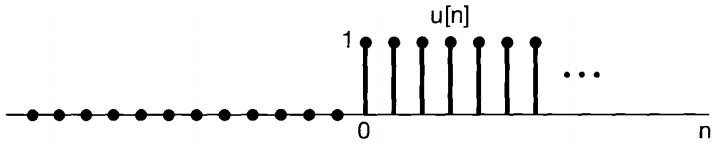
\includegraphics[width=.5\textwidth]{dcUnitStep}
	\label{dcUnitStep}
	\caption{$u[n]$}
\end{figure}
\[\delta[n]= \begin{cases} 
      0 & n\neq 0 \\
      1 & n=0 
   \end{cases}
\]
\begin{figure}[ht]
	\centering
	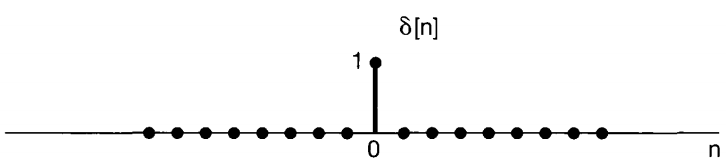
\includegraphics[width=.5\textwidth]{dcImpulse}
	\label{dcImpulse}
	\caption{$\delta[n]$}
\end{figure}
% maybe someday add pictures
The discrete time impulse function presents a "sifting feature" in that when integrated (or rather, summed) it can "sift" out a specific point.
$$\sum_{t=-\infty}^\infty x(t)\delta(t)=x(0)$$
And more generally,
$$\sum_{t=-\infty}^\infty x(t)\delta(t-k)=x(k)$$

\begin{figure}[ht]
	\centering
	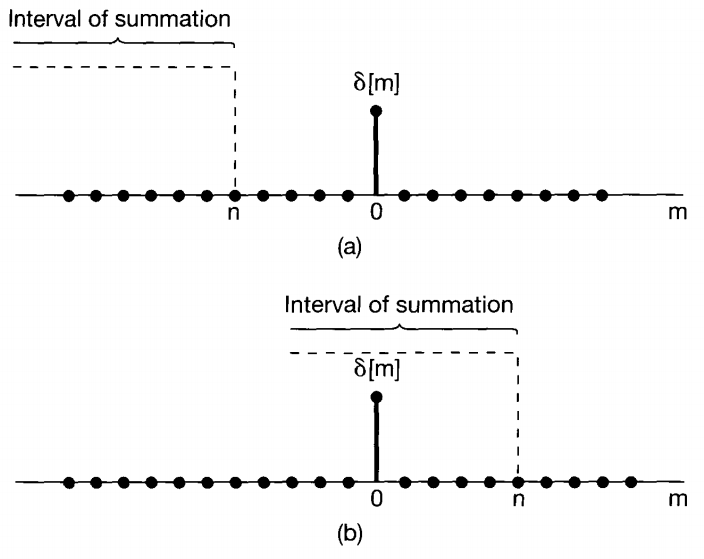
\includegraphics[width=.5\textwidth]{dcImpulse-Shifting}
	\label{dcImpulse-Shifting}
	\caption{$\delta[n]: Sifting$}
\end{figure}
\subsection{Continuous Time}
In continuous time, things are a bit more hairy.
The unit step function is defined as such:
$$u(t)=\begin{cases} 0, & t < 0, \\ 1, & t \ge 0, \end{cases}$$ 
Further, a second, more useful definition is as the derivative of the ramp function:
$$u(t) = \frac{d}{dt}r(t)$$
\begin{figure}[ht]
	\centering
	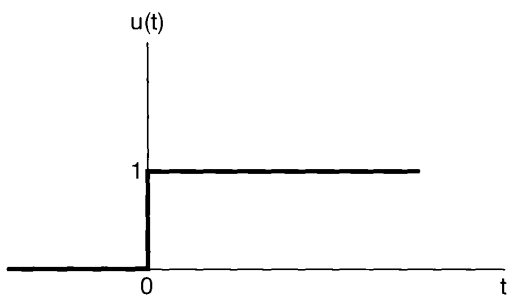
\includegraphics[width=.5\textwidth]{ctUnitStep}
	\label{ctUnitStep}
	\caption{$u(t)$}
\end{figure}
The impulse function is defined in terms of the unit step function:
$$u(t)=\int_{-\infty}^t \delta(\tau) d\tau\quad\rightarrow\quad \frac{d}{dt}u(t)=\delta(t)$$
Further, this gives us that the impulse function is the second derivative of the ramp function:
$$\delta(t)=\frac{d}{dt}u(t)=\frac{d^2}{d^2t}r(t)$$
Much like DT impulse function, the CT impulse function also has sifting properties:
$$x(t)\delta(t)=x(0)\delta(t) \qquad x(t)\delta(x-k)=x(k)\delta(x-k)$$
$$\int_{-\infty}^\infty x(t)\delta(t-k) dt = x(k)$$
\section{System Classifications (Again)}
\define{Memory}{A system is said to be memoryless if its output for each value of the independent variable at a given time is dependent only on the input at that same time. For example, the system specified by the relationship:
$$y[n]=2x[n]+x[n]^2$$
is memoryless, as the value of $y[n]$ at any particular time $n$ depends only on the value of $x[n]$ at that time.
An example of a system with memmory is a summer or accumulator:
$$\sum_{k=-\infty}^nx[k]$$}

\define{Invertible System}{A system is invertible if for every $H(x(t))$ there exists a function $W$ such that $W(H(x(t)))=x(t)$ (aka $H$ is invertible)}

\define{Causal System}{A system mapping $x$ to $y$ is causal iff for any pair of inputs $x_1(t)$ and $x_2(t)$ satisfying:
$$x_1(t) = x_2(t), \forall t\leq t_0$$
the corresponding outputs satisfy
$$y_1(t) = y_2(t), \forall t\leq t_0$$}
\section{Convolution}
The convolution is defined as follows:
$${\displaystyle {\begin{aligned}(f*g)(t)&\,{\stackrel {\mathrm {def} }{=}}\ \int _{-\infty }^{\infty }f(\tau )g(t-\tau )\,d\tau \\&=\int _{-\infty }^{\infty }f(t-\tau )g(\tau )\,d\tau .\end{aligned}}}$$
	It is commonly written as:
$${\displaystyle f(t)*g(t)\,{\stackrel {\mathrm {def} }{=}}\ \underbrace {\int _{-\infty }^{\infty }f(\tau )g(t-\tau )\,d\tau } _{(f*g)(t)},}$$
A wonderful visual explanation of this can be found on wikipedia: \url{https://en.wikipedia.org/wiki/Convolution#Visual_explanation}

The Discrete Time convolution is as one would expect:
$$x*y=\sum_{k=-\infty}^\infty x(k)y(t-k)=\sum_{k=-\infty}^\infty x(t-k)y(k)$$
\section{Impulse Response}
Let $H$ be an arbitary LTI system that takes signals $x$ to outputs $y$ like this:
$$H[x[t]]=y[t]$$
From before, we know that we can represent $x[t)$ as a sum of weighted signals:
$$\sum_{k=-\infty}^\infty x[k]\delta[t-k]= ... + x[-1]\delta[t+1] + x[0]\delta[t] + x[1]\delta[t-1] + ... $$
So, 
$$H[x[t]]=H[... + x[-1]\delta[t+1] + x[0]\delta[t] + x[1]\delta[t-1] + ...] = y[t]$$
Furhter, since $H$ is linear, it follows that:
$$H[x[t]]= ... +H[ x[-1]\delta[t+1]] + H[x[0]\delta[t]] + H[x[1]\delta[t-1]] + ... = y[t]$$
And, since $x[-1]$ and the like are constants:
$$H[x[t]]= ... +x[-1]H[\delta[t+1]] + x[0]H[\delta[t]] + x[1]H[\delta[t-1]] + ... = y[t]$$
Finnaly, since $H$ is time-invarient:
$$H[x[t]]= ... +x[-1]H\Big[\delta[t]\Big][t+1] + x[0]H\Big[\delta[t]\Big][t] + x[1]H\Big[\delta[t]\Big][t-1] + ... = y[t]$$
So, lets let $H\Big[\delta[t]\Big][t] = H_\delta[t]$ This is called the systems \textbf{impulse responce} (the system's responce to an impulse - go figure)
$$\sum_{k=-\infty}^\infty H_\delta[t-k]x[k]$$
Notice anything?
$$\sum_{k=-\infty}^\infty H_\delta[t-k]x[k]=H_\delta[t]*x[t]$$
By finding a LTI systems impulse responce, we know how it will react to any signal. 

Some useful facts:
$$a(t)*(b(t)+c(t)) = a(t)*b(t)+a(t)*c(t)$$
If $y_1$ and $y_2$ are the outputs of two sytems such that:
$$y_1(t)=x(t)*h_1(t)$$
$$y_2(t)=x(t)*h_2(t)$$
Then the system $y(t)=y_1(t)+y_2(t)$ has impulse response $h_1(t)+h_2(t)$:
$$y(t)=y_1(t)+y_2(t) = x(t)*h_1(t)+x(t)*h_2(t)= x(t)*(h_1(t)+h_2(t))$$
The associative property also holds:
$$a(t)*(b(t)*c(t))=(a(t)*b(t))*c(t)$$
\section{ADD TITLE HERE?}
\define{Rise time}{the time taken by a signal to change from a specified low value to a specified high value}
\section{Fourier Series}
$$s(x)=\overbrace {\frac{a_{0}}{2}} ^{A_{0}}+\sum_{n=1}^{\infty}\left(a_{n}\sin(\phi _{n})\cos \left({\tfrac {2\pi nx}{P}}\right)+b_{n}\cos(\phi _{n})\sin \left({\tfrac {2\pi nx}{P}}\right)\right)$$
Where $s(x)$ is the fourier series approximation of a function with period $P$ and:
$$a_{n}={\frac {2}{P}}\int _{x_{0}}^{x_{0}+P}s(x)\cdot \cos \left({\tfrac {2\pi nx}{P}}\right)\ dx$$
$$b_{n}={\frac {2}{P}}\int _{x_{0}}^{x_{0}+P}s(x)\cdot \sin \left({\tfrac {2\pi nx}{P}}\right)\ dx$$
However, there is also a complex exponential based version of the form:
$$s(x)=\sum_{n=-\infty}^\infty c_n\cdot e^{i\frac{2\pi nx}{P}}$$
where $P$ is the period, and
$$c_n=\frac{1}{P}\int_{x_0}^{x_0+P}s(x)\cdot e^{-i\frac{2\pi nx}{P}} dx$$
Further, because there are apparently \textit{only two letters in the alphabet}:
$$A_k = 2Re(c_n)\qquad B_k = -2Im(c_n)$$%https://engineering.purdue.edu/ME365/Textbook/chapter8.pdf


Also helpful: $e^{ix}=\cos x+i\sin x$

For a rectangular pulse train we see that:
\[c_n=\begin{cases}
	\frac{1}{P}\int_{x_0}^{x_0+P}y(t) dt & n=0 \\
	\frac{T_p}{P}sinc \left(\frac{nT_p}{P}\right) & n\neq0
\end{cases}
\]
where
$$sinc(x)=\frac{sin(\pi x)}{\pi x}$$

\end{document}
